\section{Simulator implementation}
\label{sec:app:simulator}

\subsection{Package overview}
The simulator has been implemented as a Python package and is available at~\cite{qoala2023simulator}.
It is divided into three subpackages: (1) \texttt{lang}, defining the format of Qoala programs and of the EHI, (2) \texttt{runtime} defining common types for the runtime system, and (3) \texttt{sim} containing Netsquid objects that implement the Qoala runtime.

The division into subpackages is made in such a way that only \texttt{sim} depends on (imports from) Netsquid; the other two subpackages are implementation independent.
The \texttt{lang} can be used standalone in a compiler, without having the compiler to depend on the runtime implementation, whether that is in simulation or on real hardware.


\subsection{Netsquid: Protocols, Components, and Listeners}
The Qoala simulator make heavy use of Netsquid's \textit{Protocol} class,
which can be used to model concurrent software systems. 
Each protocol defines its own run function, and the Netsquid simulator
executes the run functions of each protocol concurrently.
(Netsquid uses only a single thread, but protocols are run interleaved, i.e. NetSquid provides provides an asynchronous runtime).

The simulator implements a hierarchy of protocols. 
Each node in the network is a protocol, containing subprotocols for a \textit{Host, Qnos, and Netstack}. The Host represents the CPS, and the Qnos and Netstack together represent the QPS, where Qnos handle local quantum processing, and the Netstack handles requests to the central network controller. 

The protocol objects implement the runtime logic of the subsystems.
The Netsquid \textit{Component} holds static information about the subsystem, and contains \textit{Ports} for communicating with other components. Protocols use these ports to send messages to other protocols. 

Listener objects are a feature of the Qoala simulator that are protocols with the sole purpose to wait for any incoming messages on a port and then notifying the corresponding protocol of them.

\subsection{Interfaces and configuration}
The Qoala simulator allows for a lot of configuration.
The Low-level Hardware Interface (LHI) defines a format for defining physical quantum instructions, durations, and noise models.
Default values are provided for NV-centers and Trapped Ion, but custom hardware models can easily be added.
The LHI allows for representing real-life validated hardware, but also for simulating hardware that does not (yet) exist.

The LHI allows for the configurations of
\begin{itemize}
    \item Allowed gate types, gate durations, and gate noise models
    \item Qubit decoherence model and qubit topology in a node
    \item Topology of the network
    \item Entanglement fidelity and generation duration between pairs of nodes
    \item Classical communication latency between nodes
    \item Internal communication latency between scheduler components
    \item Duration of CPS instructions and of classical QPS instructions
\end{itemize}

The Native-To-Flavour (NTF) interface is used to define the translation from LHI physical quantum instructions to a NetQASM flavour.
The QPS is expected to provide an implementation of the NTF, such that it can translate instruction in Local Routines (which are from a particular NetQASM flavour) into the corresponding hardware instructions.

The Exposed Hardware Interface (EHI) is described in Section~\ref{sec:architecture}.
The simulator provides automated tools for translating a combination of an LHI instance and a NTF into an EHI.

\subsection{Simulator Architecture}
The simulator defines various component and protocol classes representing the concepts defined in Section~\ref{sec:architecture}. These classes can be instantiated in a custom way, and can hence be seen as building blocks. The simulator provides a default way of using these blocks (namely, in the way explained in the Qoala architecture), but it is possible to use these blocks in another way to investigate different architectures.
In Figure~\ref{fig:app:simulator} a schematic overview of the most important classes and their roles is given, and in Figure~\ref{fig:app:simulator_sequence} an overview is provided of the general sequence of actions involved when simulating the execution of one or more applications on a quantum network.


\begin{figure*}[hp]
    \centering
    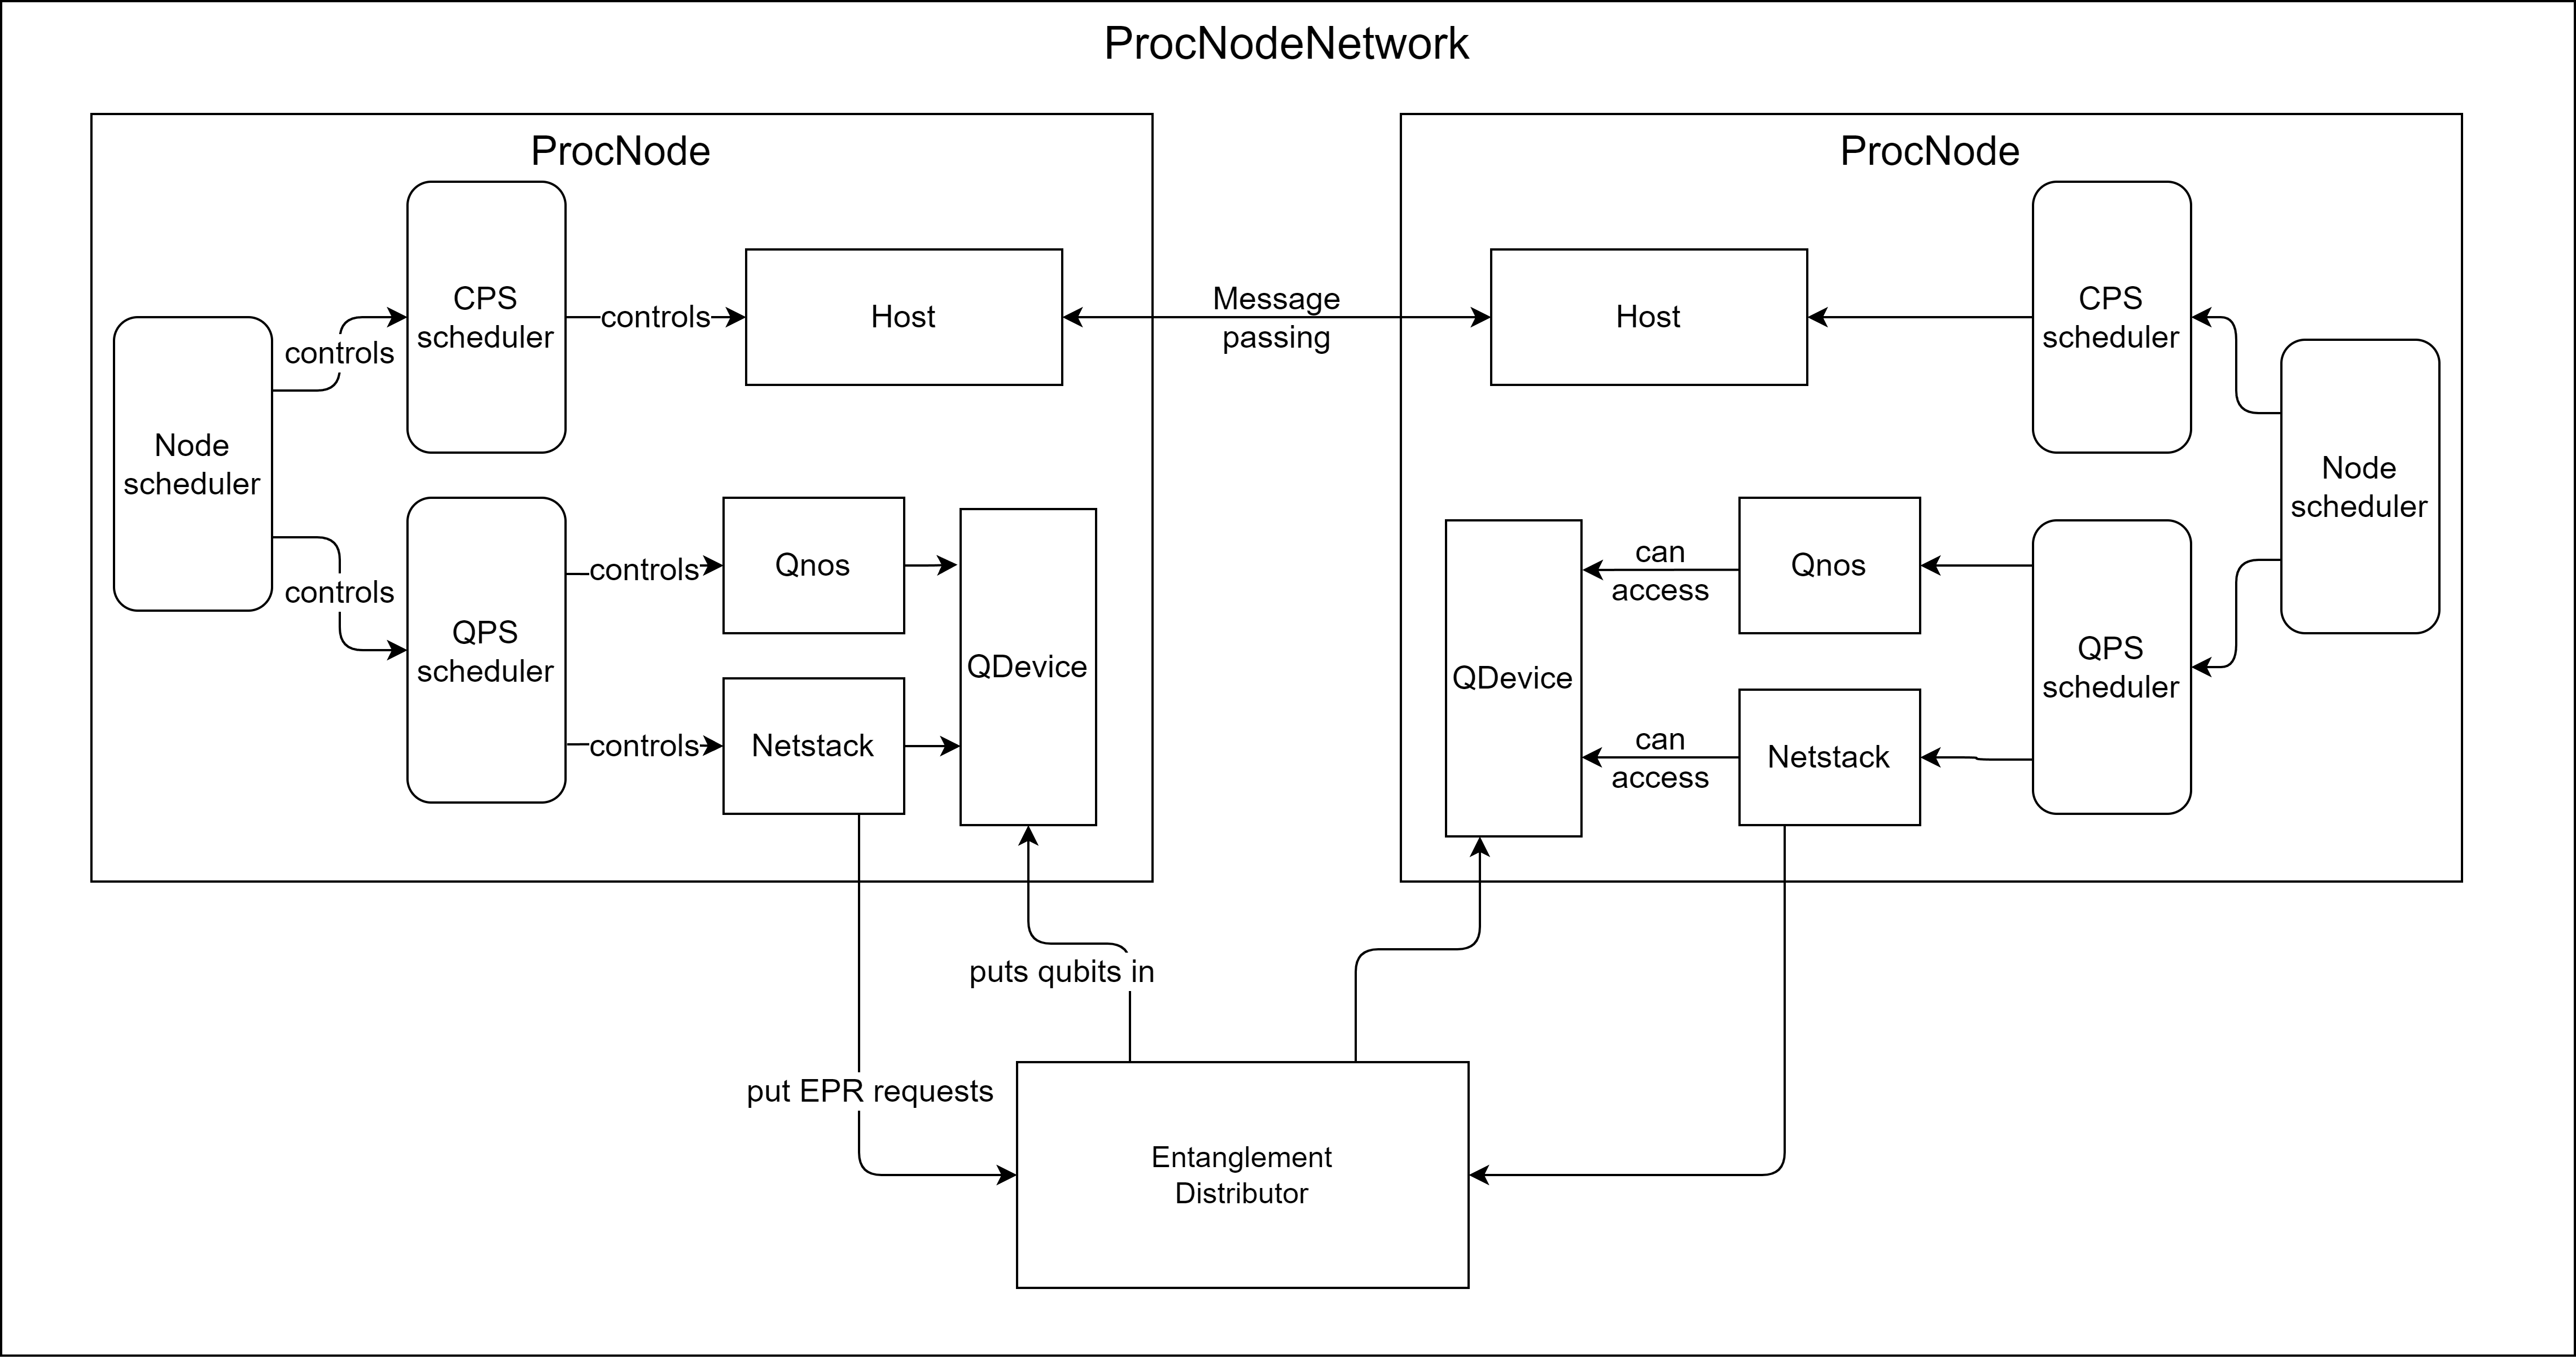
\includegraphics[width=\textwidth]{figures/qoala/simulator.png}
    \caption{High-level overview of the simulator architecture. Each box represents a component.
    A single network component can contain multiple nodes (two are shown, but there can be more).
    Each node contains a node scheduler, CPS scheduler and QPS scheduler, implementing the algorithms as described in Appendix~\ref{sec:app:scheduling_execution}.
    A single entanglement distributor object creates entangled pairs and puts the qubits directly in the quantum memory of the nodes, in the QDevice.
    }
    \label{fig:app:simulator}
\end{figure*}

In our simulator, the network controller (Appendix~\ref{sec:app:entanglement_distribution})
is implemented as a single centralized entity called EntDist (Figure~\ref{fig:app:simulator}).

\begin{figure*}[hp]
    \centering
    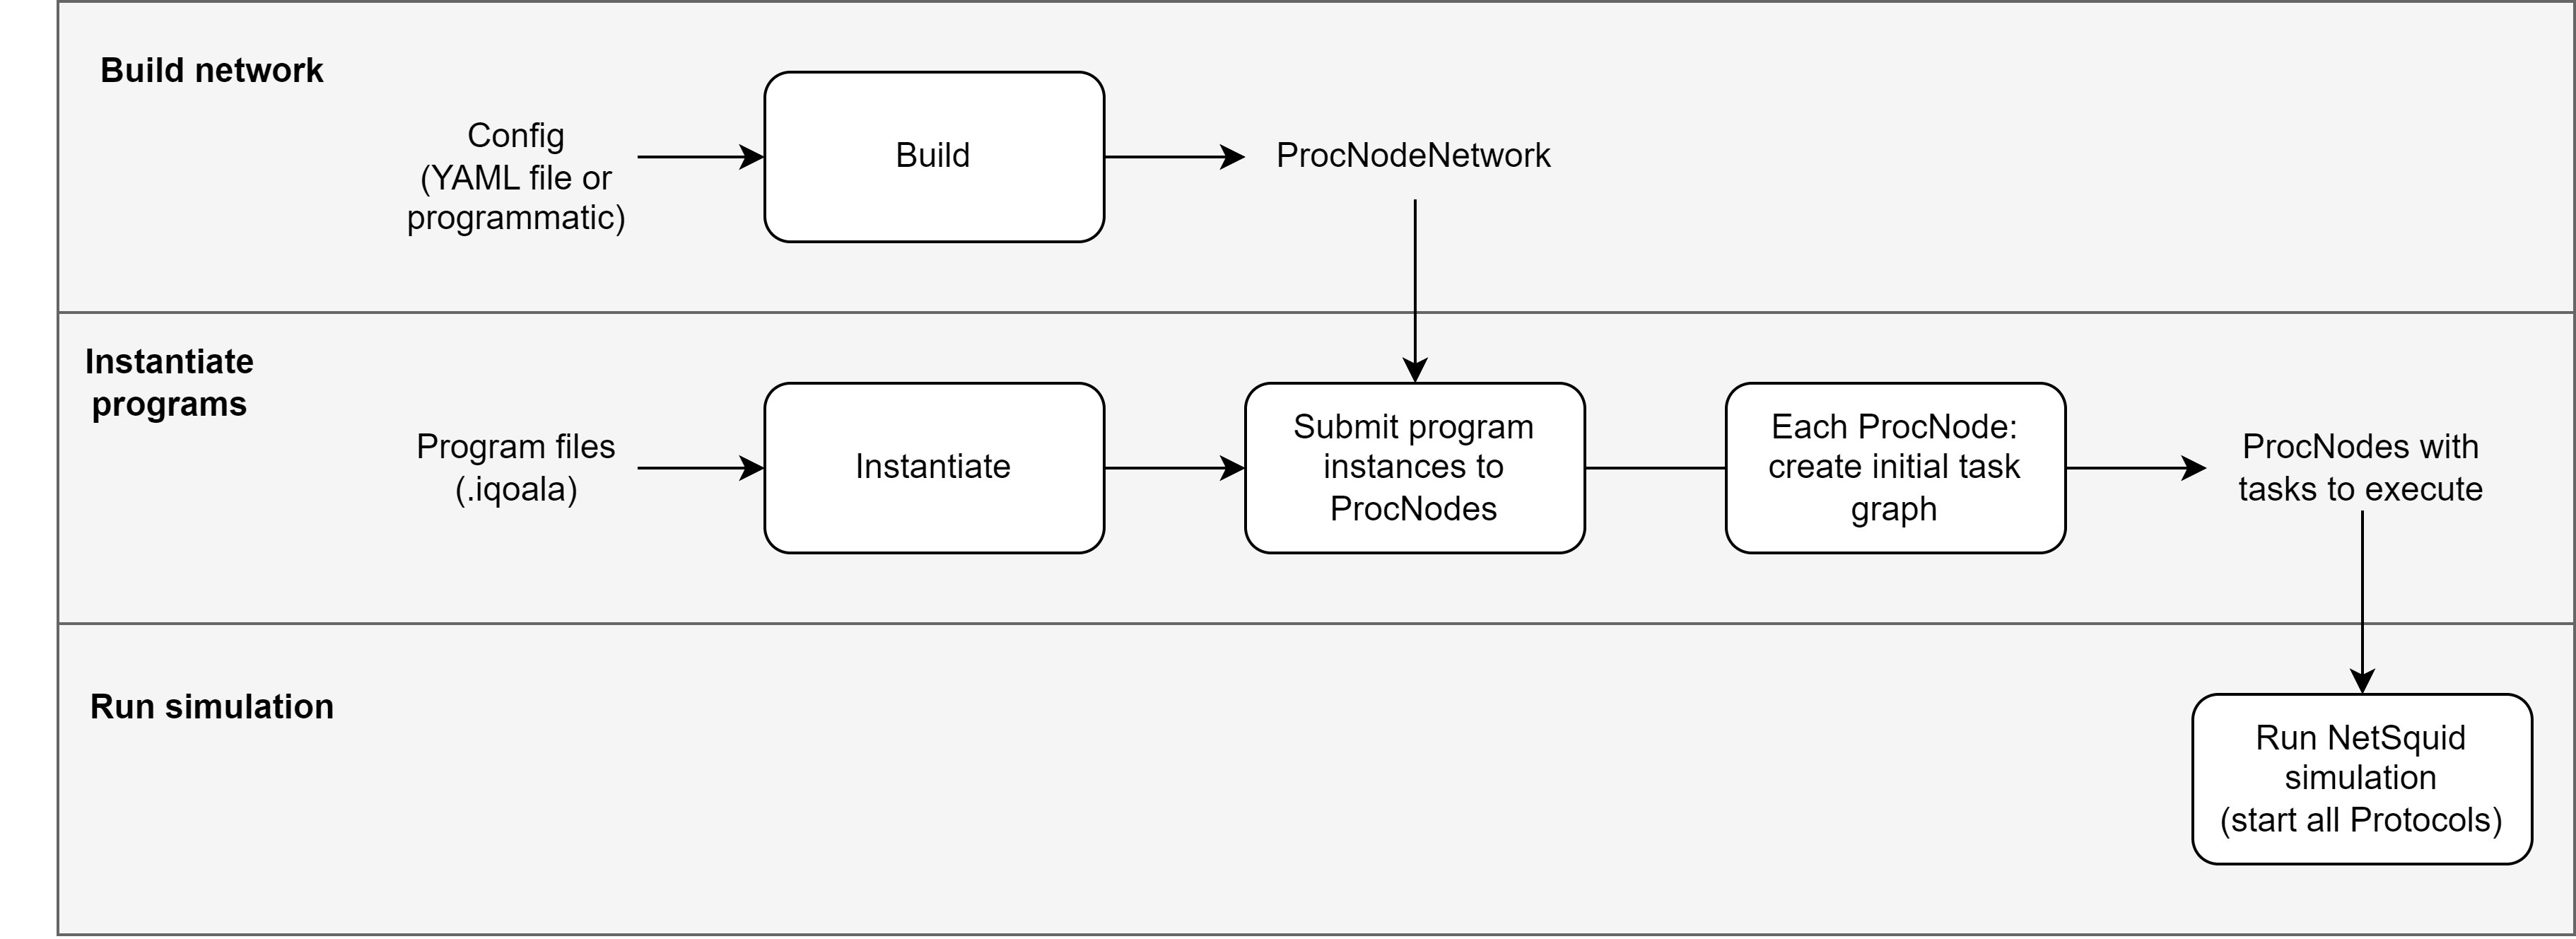
\includegraphics[width=\textwidth]{figures/qoala/simulator_sequence.png}
    \caption{High-level overview of sequence of steps performed in order to simulate a network running programs on nodes implemented Qoala.
    }
    \label{fig:app:simulator_sequence}
\end{figure*}


